\documentclass[conference]{IEEEtran}
\IEEEoverridecommandlockouts
\renewcommand{\refname}{Bibliografía}
% The preceding line is only needed to identify funding in the first footnote. If that is unneeded, please comment it out.
\usepackage{cite}
\usepackage{amsmath,amssymb,amsfonts}
\usepackage{algorithmic}
\usepackage{graphicx}
\usepackage{textcomp}
\usepackage{xcolor}
\usepackage{url}
\usepackage{upgreek}
\usepackage{amssymb}
\usepackage{verbatim}
\def\BibTeX{{\rm B\kern-.05em{\sc i\kern-.025em b}\kern-.08em
    T\kern-.1667em\lower.7ex\hbox{E}\kern-.125emX}}
\begin{document}

\title{Proyecto 2\\
{\footnotesize \textsuperscript{}IC3002 - Análisis de Algoritmos}
{\footnotesize \textsuperscript{}Profe.: Yuen Law Wan}
{\footnotesize \textsuperscript{}I Semestre 2020}
}

\author{\IEEEauthorblockN{Joseph Tenorio Pereira}
\IEEEauthorblockA{\textit{2019064588} \\
}
\and
\IEEEauthorblockN{Jose Pablo Muñoz Montero}
\IEEEauthorblockA{\textit{2019061904} \\
}
}

\maketitle

\begin{abstract}
The following documentation revolves around the creation and analysis of a Monte Carlo path tracing algorithm for two dimensional images. This algorithm is based on starting with a black canvas and casting light rays out of every pixel in the canvas. The path of these rays will be followed, and by combining its reference color with the color of every surface it bounces on, the distance it travels, and the color of the light source reached, the correct color value will be assigned to each pixel. Since this is a Monte Carlo algorithm, the accuracy of the render is considered a “bet”, since it varies with every try and improves by increasing the resources used. Nevertheless, several methods of optimization were applied, such as dynamic programing. To begin, a brief introduction on path tracing will be provided. Next, the thought process behind the algorithm will the thoroughly explained. Additionally, several rendered results will be presented to demonstrate the accuracy of the algorithm with varying parameters. Last, conclusions will be drawn. 
\end{abstract}

\section{Introducción}

El renderizado o síntesis de imágenes es entendido, según \cite{b1}, como la creación de imágenes fotorrealistas o no fotorrealistas a partir de un modelado en dos o tres dimensiones y por medio de un programa informático. La simulación del comportamiento de la luz es un componente clave en el renderizado de imágenes a partir de escenarios virtuales, ya que la iluminación es uno de los primeros aspectos que institivamente analizamos a la hora de evaluar la calidad de una imagen. En la realidad, las fuentes de luz libera una cantidad inmensa de rayos de luz, es decir, fotones, en todas las direcciones, de modo que algunos de estos rayos rebotan en los objetos que vemos y algunos de esos rayos rebotados alcanzan nuestros ojos. Es por medio de este mecanismo físico que somos capaces de apreciar el fénomeo de la iluminación a través de nuestros ojos. Asimismo, simular dicho mecanismo ha sido uno de los principales retos para la síntises de imágenes asistida por computadora, tanto en términos de la calidad obtenida como de los recursos requeridos para el renderizado, en otras palabras, en términos de eficiencia.

Uno de los métodos más usados simular la iluminación y otros detalles en el renderizado de imágenes corresponde a la rasterización (del término en inglés \textit{rasterizing}). A grander rasgos, en dicho proceso una imagen inicialmente almacenada como una serie de objetos geométricos dependientes tales como círculas o curvas, conocida como imagen vectorial, es transformada en un mapa de bits o imágen ráster, la cual corresponde al resultado de la renderización. Como se indica en \cite{b1}, la razón por la que la rasterización es de los métodos más usados yace en la rapidez con la que se pueden sintetizar las imágenes, no obstante, se requieren de técnicas muy avanzadas para lograr aumentar la calidad de una imagen producida por \textit{rasterizing}, en especial en cuanto a la iluminación. Debido a esto último, es que métodos de \textit{Ray Tracing}, tales como el \textit{Path Tracing}, se suelen usar para obtener simulaciones con comportamientos luminícos más realistas. 

El término \textit{Ray Tracing} engloba a una amplia gama de algoritmos encargados de simular la iluminación de una síntesis de imagen. En general, \cite{b1} nos indica que los \textit{Ray Tracers} generan rayos de luz desde algún punto o píxel en específico y estiman su comportamiento conforme el mismo encuentra sus objetos en su camino. Dicho comportamiento puede incluir reflexión para ilmunación global, refracción, transparencia, etc. En el caso de la reflexión de los rayos, dado que estos pueden técnicamente interactuar con los objetos un número ilimitado de veces, además de que la cantidad de rayos a seguir crece exponensialmente conforme estos van interactuando con los objetos, se suele establecer algún mecanismo para limitar la cantidad de rayos. Lo anterior se relaciona con el hecho de que si bien los \textit{Ray Tracers} suelen permitir una calidad muy superior a la de un \textit{rasterizer}, los primeros suelen requerir mucho más tiempo y recursos, razón por la cual se concibió un tipo de \textit{Ray Tracer} que gracias un modelo de algoritmo de Monte Carlo es capaz de alcanzar calidades similares a las de los demás \textit{Ray Tracers} con menos recursos y tiempo: el \textit{Path Tracing}.

Los \textit{Path Tracers} corresponden a un tipo de \textit{Ray Tracing} en el que cuando un rayo encuentra una superficie no se crean todos los posibles rayos que surgirían a consecuencia del rebote. En su lugar, un  \textit{Path Tracer} crean un número variable de rayos en direcciones de rebote válidas pero aleatorias. Es por lo anterior que los \textit{Path Tracers} requieren menos tiempo y recursos para operar, ya que siguen una cantidad de rayos mucho menor en comparación con los demás \textit{Ray Tracers}. La calidad del renderizado final se mantiene, de acuerdo al modelo de los algoritmos Monte Carlo, por medio de la promediación de los rayos generados para cada punto, además, dichos rayos son conocidos como muestras y su cantidad constituye el párametro de recursos a usar típico de los algoritmos de Monte Carlo. Como último dato respecto al \textit{Path Tracing}, existen dos formas de crear y seguir los rayos generados por el algoritmo, en la primera los rayos son generados en las fuentes de luz y van interactúando con los objetos hasta acabar aleatoriamente en un píxel, en la segunda, se crean los rayos desde cada pixel y se les sigue hasta que lleguen a una fuente de luz, y desde ahí se traza el camino a la inversa para calcular la luz que llegará al píxel. Dicho todo lo anterior, el objectivo del presente proyecto es el desarrollo de un renderizador de imágenes que calcule la iluminación directa por medio de un \textit{Ray Tracer} y la indirecta con un \textit{Path Tracer}. Además, se busca que la simulación de la iluminación incluya el efecto de \textit{Color Bleeding}, es decir, que el color de un objeto en la imagen influya el color final de las superficies que le rodean.

\section{Trabajo Relacionado}

Cómo ya se mencionó al principio de este documento, \textit{Ray Tracing} incluye un amplio espectro de técnicas para seguir el comportamiento de luz, dentro de las cuales figura el uso de reflexiones y refracciones recursivas. Dicha implementación de la recursividad en \textit{Ray Tracing} se encuentra más desarrollada y descrita en \cite{b2}, y es por eso que el presente para el presente proyecto se implementaron las reflexiones de la luz con un modelo recursivo basado en el encontrable en dicha fuente. Cabe resaltar que las reflexiones y refracciones recursivas son de particular utilidad para el  \textit{Path Tracing} ya que facilitan la limitación de las interacciones que un rayo puede tener con los objetos de la imagen,por ejemplo, al rebotar un máximo de veces antes de descartar la muestra. Ahora bien, \cite{b2} también realiza un repaso de las propiedades y fórmulas ópticas involucradas en la reflexión y refracción, todo orientado a la simulación de dicho fénomeno en un \textit{Ray Tracing}, lo cual fue muy útil a la hora del diseño de las funciones de rebotes aleatorios y rebotes especulares que usa el \textit{Path Tracer} del proyecto.

En cuanto a la programación del \textit{Path Tracer} como tal, uno de los efectos ópticos deseados en el renderizado del mismo es el de \textit{Color Bleeding}. Para lo anterior se consultaron los trabajos encontrables en \cite{b3} y \cite{b4}, en los cuales se inspiró la combinación de colores RGB presente en el proyecto. En nuestro caso, dicha combinación ocurre cuando un rayo rebota en una superficie, ya que el color del píxel en el que se reboto es combinado con el color del píxel de origen.

\section{Métodos}
Primeramente, cabe resaltar que la solución aquí descrita se implementó en un programa realizado en el lenguaje Python, en su versión 3.7 y por medio del ambiente de desarrollo PyCharm. Además, aparte de varias librerías estándar de Python, también se incorporaron los módulos de Pygame, Numpy y Pillow a dicho ambiente. A continuación se dará una explicación detallada del algoritmo utilizado para iluminar la imagen. Para comenzar, la técnica elegida fue recorrer cada pixel de la imagen e ir asignándole a estos su color calculado. Para el cálculo del color de cada pixel individual el algoritmo se dividirá en tres secciones para facilitar su compresión. La primera siendo un \textit{Ray Tracer} que se encarga de calcular la iluminación directa para cada pixel. La segunda un \textit{Path Tracer} para calcular la iluminación indirecta y color bleeding para cada pixel. Y la tercera una serie de funciones geométricas para calcular el camino de los rayos de luz utilizados en las secciones anteriores. Para finalizar, se discutirá la optimización implementada. 

Antes de comenzar es importante aclarar las estructuras de los objetos utilizados en el programa. Primero, los colores todos se interpretan como su valor RGB en una lista de tres elementos. Segundo, las figuras geométricas en la imagen (en este caso paredes) se crean a partir de un objeto línea que consiste de dos puntos (x, y), el programa solo implementa líneas rectas ya sean horizontales, verticales o inclinadas. Tercero, las fuentes de luz pueden ser un único punto o una línea. Los rayos de luz se representan mediante un objeto rayo que consiste de un punto (x, y) del cual parte y un segundo punto que indica su dirección infinita, este punto se calcula a partir de un ángulo de dirección. Además, el vector es normalizado para simplificar los cálculos. Por último, la imagen de referencia y la imagen a pintar fueron traducidas a matrices de \textit{Numpy} que se componen por listas con los valores RGB de cada pixel. 

La primera sección del algoritmo encargada del cálculo de la iluminación directa comienza con el color en negro. Siguiente, se hace un ciclo para cada fuente de luz que se esté utilizando. Dentro de este ciclo se crea una línea recta del pixel actual a la fuente de luz actual y se le calcula la distancia mediante el teorema de Pitágoras. Luego, se debe revisar si existe alguna pared que interseque dicha línea. Esto se verifica mediante un ciclo para todas las paredes creadas, dentro del cual se busca un punto de intersección utilizando los determinantes y por medio del método encontrado en \cite{b3}. Cabe resaltar que no se toman en cuenta las paredes transparentes. Si existiera algún punto de intersección el ciclo se interrumpe y el color del pixel se mantiene en negro. Si no existe ningún punto de intersección se procede a calcular la intensidad de la luz directa con la distancia calculada y la ley de la inversa del cuadrado vista en \cite{b4}. Además, se obtiene el color de la imagen de referencia para el pixel actual. El color final es la multiplicación del color de referencia, el color de la fuente de luz y la intensidad calculada. De esta forma los colores se van sumando para cada fuente de luz, y al terminar el ciclo se promedia entre la cantidad de luces, así queda el pixel con su color de iluminación directa asignado. 

A continuación, es necesario calcular si el pixel actual recibe luz indirectamente a través de rayos que rebotan en las paredes establecidas y llegan a él. Estos pueden venir de las mismas fuentes que lo iluminan directamente, o inclusive de alguna que no lo ilumina directamente. Adicionalmente, al rebotar, estos rayos llevan con ellos un poco del color de la pared en que rebotaron y lo pasan al pixel de destino como parte del efecto de \textit{Color Bleeding}. Esta sección del algoritmo es un algoritmo de Monte Carlo y se basa en lanzar rayos en direcciones aleatorias desde el pixel actual y seguir su camino para verificar si proveen iluminación indirecta. Por ser un método de Monte Carlo debe contar con un parámetro de entrada que se refiere a la cantidad de recursos que se van a utilizar, en este caso son la cantidad de rayos lanzados por pixel. La función comienza con un ciclo para la cantidad de rayos elegida, dentro de este se calcula un ángulo aleatorio de 0 a 2 * $\pi$ radianes (un ciclo completo). Luego, se crea un rayo con dicho ángulo y se llama una función recursiva con ese rayo para seguir su camino. Es importante mencionar que la función recursiva utiliza otro parámetro de entrada que se refiere a la cantidad de rebotes realizados, con tal de poder especificar un máximo y anular el rayo o direccionarlo intencionalmente a la fuente de luz.

La función recursiva comienza preguntando por su condición de parada, es decir, si la cantidad máxima de rebotes no ha sido superada. Como no es el caso, se procede a revisar si el rayo interseca alguna pared en su camino. Esto se verifica con un ciclo para todas las paredes existentes y la misma fórmula de determinantes utilizada anteriormente y encontrada en \cite{b2} la cual además retorna la distancia a la intersección. Sin embargo, en este caso si es necesario completar el ciclo ya que se debe obtener la intersección más cercana, la que retorna la menor distancia. Si no existe ninguna intersección la función recursiva retorna el color negro, ya que el rayo no aporto ningún color. Si existiera una intersección se calcula la intensidad de la luz que proviene de ese rebote con la distancia y la ley de la inversa del cuadrado vista en \cite{b4}. Además se obtiene el color de la imagen de referencia para el pixel del cual partió el rayo. Por último, la función retorna el color bleeding producido por el rayo lanzado: la multiplicación de la intensidad, el color de referencia y el color entrante de donde ocurrió el rebote.

Antes de poder retornar se debe calcular el color entrante recursivamente. Para esto se crea un nuevo rayo a partir de donde ocurrió el rebote, el cual puede tener tres comportamientos diferentes. Si el rebote ocurrió en una superficie especular se obtiene un rayo con una dirección basada en el ángulo correcto de reflexión. Si el rebote ocurrió en una superficie no especular se obtiene un rayo con una dirección totalmente aleatoria, basada únicamente en no atravesar el segmento donde reboto. Por último, si el rebote ocurrió en una superficie no especular pero el siguiente rayo es el último de acuerdo al máximo, se obtiene un rayo direccionado específicamente a alguna fuente de luz accesible para no desperdiciarlo. Luego, se llama a la función recursivamente con el nuevo rayo y la cantidad de rebotes aumentada en uno, hasta llegar al último rayo permitido o hasta que el rayo no tenga ninguna intersección. 

Al llegar al último rayo según el máximo se debe revisar si el rayo interseca con una fuente de luz, ya que antes estas estaban siendo ignoradas, y luego se debe revisar si no existe ninguna pared de por medio. Para esto se utilizan los mismos cálculos mencionados anteriormente. Si el rayo no cumple con ambas condiciones la función retorna negro y recursivamente continua retornando negro hasta llegar al pixel original. Si el rayo si cumple, se obtiene la intensidad con respecto a la luz, el color de referencia y se retorna la multiplicación de estos con el color de la luz, siendo esto el color de donde ocurrió el último rebote antes de llegar a la luz. Recursivamente se van acumulando los colores de los rebotes hasta llegar al pixel original y salir de la función recursiva retornando el color final producido por el color bleeding. Esta función también acumula la distancia total recorrida por el rayo y el color de la fuente de luz a la que llego para retornarlos.

Una vez de vuelta en la función original, si el color retornado por la función recursiva es diferente de negro, este se le suma al color del pixel (el cual en este momento tiene nada más su valor de iluminación directa) y se inicia un conteo de rayos válidos, es decir, rayos que llegaron a una fuente de luz. Además, se utiliza la distancia total recorrida para calcular la intensidad de la iluminación indirecta y junto con el color de referencia y el color de la fuente de luz que se intersecó se obtiene otro color para sumar al pixel y otro rayo valido. Una vez terminado el ciclo para la cantidad de rayos deseada, el color final del pixel se calcula promediándolo de nuevo entre la cantidad de rayos válidos y se le asigna a la imagen.  

En cuanto a las funciones encargadas de crear los vectores que representan a rayos que rebotaron, estas se dividen en rebote especular, rebote dirigido y rebote aleatorio. Previo a explicar sus diferencias, cabe resaltar que los tres procedimientos crean un vector cuyo origen se ubica en el punto de intersección del rayo anterior con la superficie en cuestión. Debido a lo anterior, el grueso de los cálculos realizados tiene por objetivo determinar el ángulo a asignar al vector creado. Para evitar malentendidos, de aquí en adelante se entiende como ángulo de los vectores (o de los rayos que estos representan) a la cantidad de radianes existentes entre el límite del primer y cuarto cuadrante del plano cartesiano (mitad positiva del eje X) y la línea de rayo, esta última siendo aquella línea resultante de extender el rayo rebotado hasta el infinito en ambas direcciones. Además, se recuerda que dichos ángulos incrementan en el sentido de las agujas del reloj. También cabe resaltar que el plano cartesiano mencionado anteriormente tiene su origen en el centro de la imagen.

La primera función de rebote diseñada fue la de rebote aleatorio, la cual se emplea en aquellos rebotes que ni son el último rebote del rayo original ni se producen en superficies especulares. En este caso, el ángulo del nuevo rayo debe ser aleatoriamente escogido entre dos rangos de ángulos, cada uno con uno con un ancho $\pi$ radianes y cada uno representando uno de los lados de la superficie, es decir, el punto medio de cada rango corresponde al valor del ángulo formado por la mitad positiva del eje X y los respectivos rayos (geométricos, no de luz) perpendiculares a la superficie y con origen en el punto de rebote. En el caso de los segmentos verticales, los dos rangos posibles a usar corresponden a ] $\pi$/2, 3$\pi$/2 [ para el lado izquierdo y ] 3$\pi$/2, 2$\pi$[ $\cup$ ] 0,  $\pi$/2 [ para el derecho, por lo que solo queda comparar la posición X del origen del rayo a rebotar con el mismo valor del punto de rebote para saber de que lado del segmento se dió el rebote. De manera similar, los rangos posibles para los segmentos horizontales corresponden a ] 0, $\pi$ [ para el lado inferior y ]  $\pi$,  2$\pi$ [ para el superior, y se usa la coordenada Y para determinar de que lado se dió el rebote. Por último, los segmentos inclinados requieren de un análisis más detallado, ya que se requiere calcular en tiempo de ejecución los posibles rangos, la asignación de cada rango a un lado del segmento y el lado del segmento del que proviene el rayo a rebotar. Para todo lo anterior se debe calcular la pendiente del segmento de rebote y su ángulo menor respecto al eje de las abscisas, el cual equivale a la arcotangente de la pendiente. Tambíen se debe obtener la coordenada Y del punto de la superficie que comparte coordenada X con el origen del rayo, esto con el fin de obtener la diferencia entre las coordenadas Y del punto en la línea y del origen del rayo. Finalmente, se sabe que el rango de ángulos válido corresponde a ] arctan(pendiente), arctan(pendiente)o + $\pi$ [ si tanto la pendiente como la diferencia de ordenadas es negativa, o bien si la pendiente es negativa y la diferencia positiva. En los otros dos casos, se sabe que el rango válido corresponde a ] arctan(pendiente), arctan(pendiente) - $\pi$ [

La segunda función de rebote en programar corresponde a la de rebote dirigido. Esta función se encarga de crear un rayo de luz que se origina en el punto de rebote y apunta directamente a una fuente de luz ubicada en el lado de la superficie de rebote que el rayo impactó. Esta función es utilizada en los últimos rebotes de cada rayo originado en un píxel que no se producen en superficies especulares. El grueso de esta parte del programa se encarga de determinar que puntos de las fuentes de luz se encuentran en el lado de la superficie en el que se dió el rebote, de modo que dichos puntos son fuentes de luz candidatas para crear un rayo rebotado dirigido hacia ellas. Cabe resaltar que en esta parte del programa se ignora el hecho de si hay o no otro segmento que le impedería al rayo rebotado llegar a la fuente de luz escogida, dicha validación es realizada en la función general de \textit{Path Tracing}. En el caso de los segmentos verticales y horizontales, se realizan instrucciones similares a las presentes en el rebote aleatorio, es decir, se comparan las coordenadas X o Y del origen del rayo a rebotar y de la fuente de luz respecto a la coordenada respectiva del segmento. Si tanto la coordenada del rayo como de la fuente de luz son ambas mayores o ambas menores respecto a la coordenada del segmento, entonces el punto de la fuente de luz se considera válido, en el caso contrario, este se descarta. Similarmente, los segmentos inclinados en el rebote dirigido reutilizan el procedimiento matemático empleado en el cálculo de rebotes aleatorios para segmentos también inclinados. Se aplica exactamente el mismo procedimiento dos veces, con la diferencia de que se almacena el valor de verdad de la condición lógica en lugar de asociarla a un rango de ángulos, y que la segunda corrida del procedimiento sustituye al punto de origen del rayo con el punto candidato a ser fuente de luz válida. Independientemente del tipo de segmento en el que se da el rebote, todos los puntos de las fuentes de luz son analizados para determinar si son válidos o no. Una vez almacenadas todas las fuentes de luz válidas, se escoge una al azar y se crea una línea que pase por dicha fuente de luz y por el punto donde ocurrió el rebote, a dicha línea se le calcula el ángulo con el lado positivo del eje X y, finalmente, dicho ángulo es asignado al nuevo rayo creado. En caso de no encontrar ninguna fuente de luz válida, la muestra actual se descarta.

La tercera y última función de rebote corresponde a la utiizada cuando se trata con superficies especulares. Cabe recalcar que el objetivo de un rebote especular es que el ángulo de incidencia del rayo a rebotar sea igual al ángulo de reflexión del rayo rebotado. Al igual que con la función de rebotes aleatorios,la mayoría de las instrucciones realizadas contribuyen a determinar el ángulo en el cual se debe direccionar el nuevo rayo rebotado, cuyo origen es el punto en el que el rayo anterior intersecó al segmento especular. Dicho ángulo, en general, equivale a el ángulo del rayo incidente más $\pi$ radianes (se invierte la dirección del rayo) más o menos dos veces el ángulo de incidencia. En general, el cálculo del ángulo incidente $\theta$ se basa en la fórmula \(\theta = \arctan{(m1 - m2 / 1 + (m1 * m2))}\), donde \textit{m}1 corresponde a pendiente de la línea normal y \textit{m}2 a la pendiente de la línea de rayo. Nótose que la fórmula anterior no se puede utilizar cuando el rayo o el segmento son verticales u horizontales, por lo que para cada combinación de rayo/segmento no inclinado existe una subfunción aparte que utiliza una variante de la fórmula antes presentada o no requiere conocer el ángulo de incidencia, como es el caso de rayos verticales rebotando en segmentos horizontales. Además, que combinación de tipos de rayo/segmento se tiene determina si se suma o se resta el doble del ángulo incidente calculado. Independientemente de la subfunción usada, una vez determinado el ángulo del rayo a rebotar se crea al mismo con origen en el punto de rebote.

Finalizando, es evidente que el algoritmo cuenta con una gran cantidad de ciclos y por ende puede llegar a tener un tiempo de ejecución muy largo, como se evidenciará en los resultados. No obstante, sí fue posible encontrar optimizaciones para mejorar dicha ejecución. Primero, una optimización sencilla es el hecho de que al lanzar el último rayo de un rebote no especular este se direcciona intencionalmente hacia alguna fuente de luz. De esta forma es mucho menos probable que el rayo se desperdicie, a menos que haya una pared de por medio. Con esta optimización fue posible reducir considerablemente la cantidad de rayos necesitados para producir una imagen de buena calidad, ya que la gran mayoría de rayos terminaban siendo válidos. 

Segundo, se implementó un cierto grado de programación dinámica en el algoritmo, para evitar realizar cálculos que ya se habían realizado anteriormente. Por ejemplo, cuando el ultimo rebote de un rayo interseca una fuente de luz, se calcula el color del pixel donde ocurrió el rebote para utilizarlo en el color bleeding. Pero, este valor es a su vez el color de la iluminación directa que le provee esa fuente de luz a dicho pixel. Por ende, resulta beneficioso guardar este cálculo para no tener que volverlo a realizar cuando se vaya a calcular la iluminación directa para ese pixel. De la misma manera se debe guardar el color calculado de iluminación directa para cada pixel, para no volverlo a calcular cuando un rayo rebote en un pixel ya iluminado. Indirectamente de esta manera también se evita calcular rebotes finales que ya hayan ocurrido antes. La estructura elegida para almacenar estos colores es una matriz de tres dimensiones, igual a la matriz utilizada para guardar las imágenes, pero ahora para cada pixel (x, y) se guardan múltiples colores: los valores de iluminación directa respecto a cada fuente de luz. Así, antes de realizar cualquier cálculo de iluminación directa se debe preguntar si ya existe un valor para el pixel actual respecto a la fuente de luz actual. Esta optimización logró reducir el tiempo de ejecución del algoritmo porque los pixeles en áreas potenciales de rebotes ya no repiten cálculos.

\section{Análisis de resultados}

A continuación se mostraran varios renderizados hechos por el algoritmo, junto a los tiempos de ejecución de los mismos. Cabe resaltar que las siguientes pruebas se realizaron en un equipo con procesador Intel core i7-4790 y 16 GB de RAM y que los tiempos de ejecución se midieron mediante la librería \textit{timeit} de \textit{Python}. Para dicha medición, se crea e inicia un cronómetro estándar de \textit{timeit} al principio de la función principal de renderizado, y el mismo se detiene como última instrucción de dicha función, por lo que se puede decir que los tiempos de ejecución corresponden más específicamente al tiempo de ejecución de la síntesis de la imagen, sin tomar en cuenta instrucciones como la preparación de la ventana a mostrar o la definición de las estructuras de datos a usar. 

\begin{figure}[htbp]
\centerline{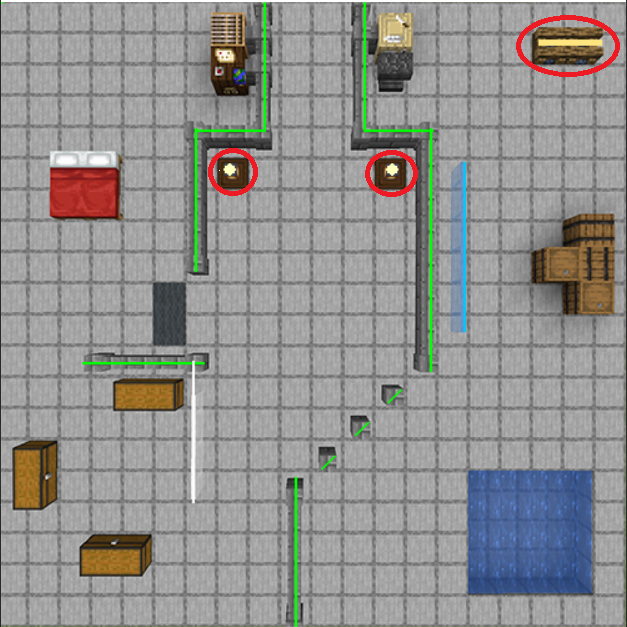
\includegraphics[scale=0.62]{Reference Image.png}}
\caption{Imagen a renderizar. Las fuentes de luz se circulan en rojo. Las superficies se resaltan en azul las especulares, blanco las transparentes y verde las regulares}
\label{Imagen de referencia}
\end{figure}

En Fig. 1 se puede apreciar la imagen que se usará de modelo para el renderizado en la mayoría de las pruebas. Nótese que la misma cuenta con 3 fuentes de luz: dos circulares y una lineal, y 13 segmentos: 11 regulares, uno transparente y uno especular. Es importante tener en cuenta la cantidad de segmentos y fuentes de luz porque estos constituyen los principales factores, aparte de la cantidad de rebotes y de muestras, en el tiempo de ejecución del algoritmo. Lo anterior se debe que los ciclos presentes en el algoritmo contarán con más iteraciones conforme se aumente el número de segmentos y fuentes de luz. También se recuerda que el algoritmo funciona con imágenes de 500x500 píxeles y que todas las pruebas aquí mostradas tienen un párametro de profundidad igual a uno.

\begin{figure}[htbp]
\centerline{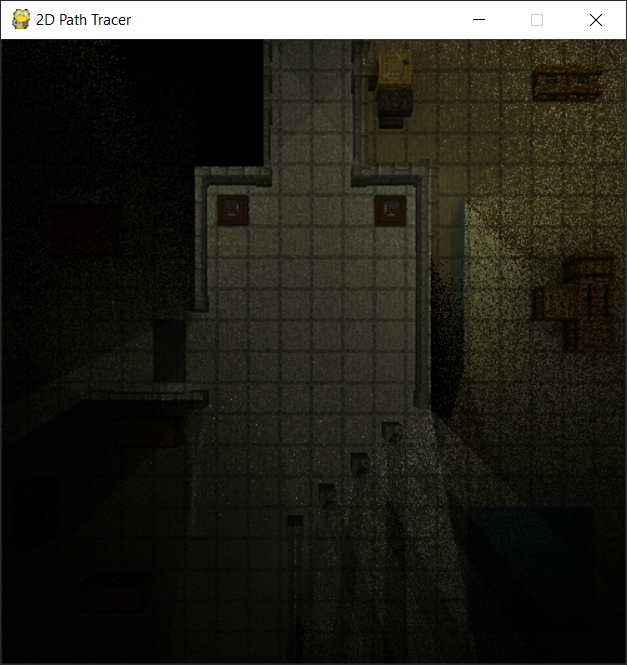
\includegraphics[scale=0.62]{Complete Lighting (50 Samples).png}}
\caption{Renderización completa con 50 muestras. Tiempo de ejecución: 16 minutos con 20 segundos.}
\label{50 muestras completo}
\end{figure}

Luego de varias corridas de prueba, se determinó que el programa genera renderizados de calidad aceptable a partir de las 50 muestras, como se puede apreciar en la Fig. 2. En la misma también se puede notar un efecto arenoso en ciertas zonas del renderizado, como el superior izquierdo o el inferior derecho de la imagen, conocido como ruido o \textit{noise}. Dicho efecto se produce debido a la baja cantidad de muestras usadas, ya que a muchos píxeles se les calculará muy pocos o ningún rayo de iluminación indirecta, lo cual los oscurece o directamente los deja en negro. Asimismo, la falta de \textit{noise} en aquellas zonas con iluminación directa evidencia el uso de \textit{Ray Tracing} para dicha tarea, ya que el mismo no se ve afectado por la cantidad de muestras usadas. La compesación de este afecto arenoso cuando se usan pocas muestras fue una de las razones por la que se decidió calcular la iluminación directa por aparte en un \textit{Ray Tracer}.

\begin{figure}[htbp]
\centerline{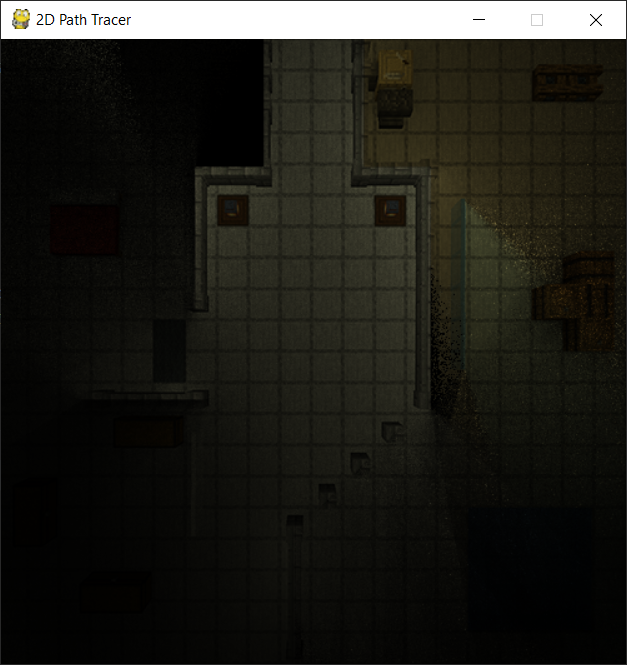
\includegraphics[scale=0.62]{Complete Lighting (225 Samples).png}}
\caption{Renderización completa con 225 muestras. Tiempo de ejecución: 1 hora con 12 minutos y 47 segundos.}
\label{225 muestras completo}
\end{figure}

\begin{figure}[htbp]
\centerline{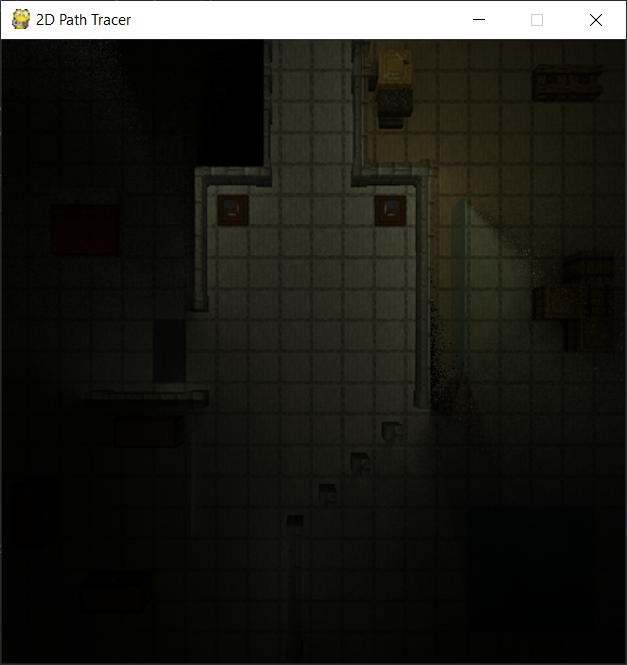
\includegraphics[scale=0.62]{Complete Lighting (500 Samples)}}
\caption{Renderización completa con 500 muestras. Tiempo de ejecución: 2 horas con 39 minutos y 21 segundos.}
\label{500 muestras completo}
\end{figure}

Una vez que se usan cantidades mayores de muestras, como en las corridas apreciables en Fig. 3 y 4, el \textit{noise} se reduce drásticamente y la transición entre zonas con iluminación directa y aquellas que solo les llega luz indirecta es más realista. No obstante, también se puede notar el considerable incremento en el tiempo de ejecución, ya que si comparamos la prueba en Fig. 3 con la de Fig. 4, hubo un aumento de aproximadamente 3 417 segundos por 175 muestras de más. Las pruebas aquí mostradas, aunadas a las que se realizaron con muchas otras cantidades, permiten estimar un aumento lineal del tiempo de ejecución conforme se aumenta la cantidad de muestras. En el caso de la imagen en Fig. 1, y ejecutando el programa en el equipo y con la profundidad dados al inicio de esta sección, se promedió un aumento de 19 segundos al tiempo de ejecución por cada incremento unitario de la cantidad de muestras. Lo anterior se puede resumir en que se puede estimar el tiempo de ejecución del algoritmo, con la imagen y condiciones especificadas,  por medio de la fórmula \(s = 19 * n\), donde \textit{s} corresponde al tiempo de ejecución en segundos y n a la cantidad de muestras. 



\begin{figure}[htbp]
\centerline{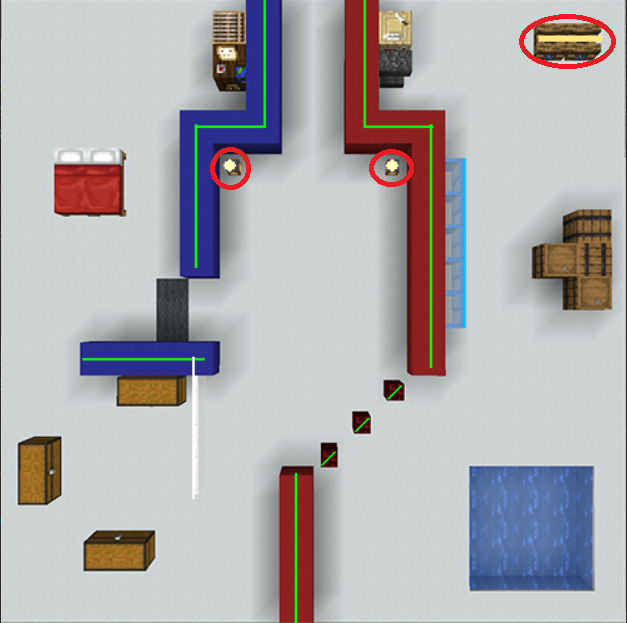
\includegraphics[scale=0.62]{Reference Image (Color Bleed).png}}
\caption{Imagen a renderizar para la prueba del \textit{Color Bleeding}. Las fuentes de luz se circulan en rojo. Las superficies se resaltan en azul las especulares, blanco las transparentes y verde las regulares}
\label{Imagen de referencia color bleeding}
\end{figure}

\begin{figure}[htbp]
\centerline{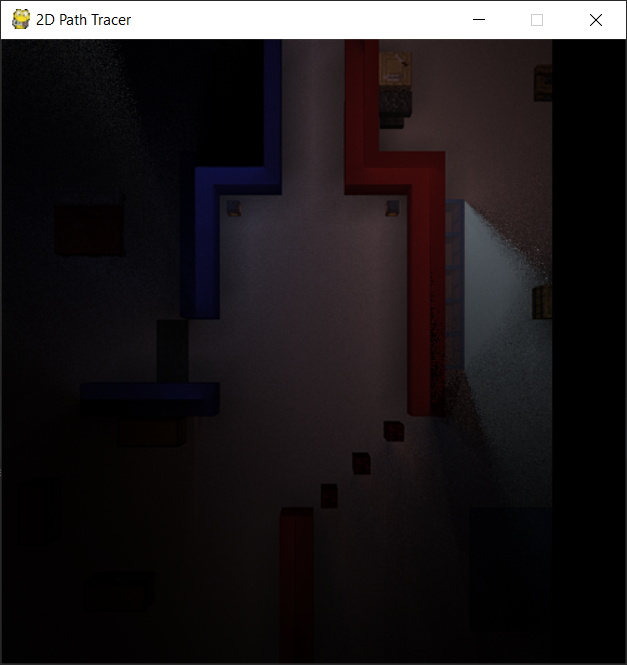
\includegraphics[scale=0.62]{Complete Lighting (500 Samples Color Bleed).png}}
\caption{Renderización para la prueba del \textit{Color Bleeding} con 500 muestras.}
\label{500 muestras color bleeding.}
\end{figure}
\section{Conclusión}

AQUI VA LA CONCLUSION

\section{Acceso al proyecto}
El repositorio de GitHub en el cual se ubican todos los archivos empleados para el desarrollo de este proyecto puede ser accesado mediante el siguiente link: \url{https://github.com/TilapiaBoi/AnalisisPRY2}

\begin{thebibliography}{00}
\bibitem{b1} https://www.online-tech-tips.com/computer-tips/what-is-path-tracing-and-ray-tracing-and-why-do-they-improve-graphics/
\bibitem{b2} https://www.cs.unc.edu/~rademach/xroads-RT/RTarticle.html
\bibitem{b3} http://graphics.stanford.edu/courses/cs348b-01/course29.hanrahan.pdf
\bibitem{b4} Wikipedia. (2020, June 08). Line–line intersection. Retrieved from https://en.wikipedia.org/wiki/Line%E2%80%93line_intersection
\bibitem{b5} Toppr. (2020, April 13). Inverse Square Law Formula. Retrieved from https://www.toppr.com/guides/physics-formulas/inverse-square-law-formula/
\begin{comment}
\bibitem{b1} J. L\'azaro, \textit{Backtracking}, Departamento de Ciencias de la Computaci\'on, Universidad de Alcal\'a, n.d. Accessed on: Mar. 18, 2020. [Online]. Available: \url{ftp://www.cc.uah.es/pub/Alumnos/G_Ing_Informatica/Algoritmia_y_Complejidad/anteriores/Apuntes/08_Backtracking.pdf}
\bibitem{b2} “Nonogram”, n.d. Accessed on: Mar. 18, 2020. [Online]. Available: \url{https://www.definitions.net/definition/Nonogram}
\bibitem{b3}  C. Wu , D. Sun, L. Chen, K. Chen, C. Kuo, H. Kang and H. Lin, "An Efficient Approach to Solving Nonograms", \textit{IEEE Transactions On Computational Intelligence And AI In Games}, vol. 5. no. 3, Sept. 2013,  pp. 251-264. Accessed on: Mar. 18, 2020. [Online]. Available: \url{http://perpustakaan.unitomo.ac.id/repository/An Efficient Approach to Solving Nonograms.pdf}
\bibitem{b4} Tech With Tim, \textit{Python Sudoku Solver Tutorial with Backtracking p.2}, Apr. 4, 2019. Accessed on: Mar. 18, 2020. [Video file]. Available: \url{https://www.youtube.com/watch?v=lK4N8E6uNr4&t=844s}
\bibitem{b5} M. Richards, \textit{Backtracking Algorithms in MCPL using Bit Patterns and Recursion}, Computer Laboratory, University of Cambridge, Feb. 23, 2009. Accessed on: Mar. 18, 2020. [Online]. Available: \url{https://www.cl.cam.ac.uk/~mr10/backtrk.pdf}
\end{comment}
\end{thebibliography}
\end{document}